\documentclass[10pt]{article}
\usepackage[a4paper,margin=2cm]{geometry}
\usepackage{amsmath,amssymb}
\usepackage{graphicx}
\usepackage{xcolor}
\usepackage{booktabs}
\usepackage{siunitx}
\usepackage[font=small,labelfont=bf]{caption}
\usepackage{float}
\usepackage{microtype}
\usepackage[pdftitle={dC_l/domega_m at fixed theta_s: emulators vs CLASS},colorlinks=true,linkcolor=blue!50!black,citecolor=blue!50!black]{hyperref}
\sisetup{table-number-alignment=center, round-mode=none}
\newcommand{\thetafid}{1.0419693546}
\newcommand{\slope}{-3.523928}
\newcommand{\sexact}{-0.74773}
\newcommand{\spipe}{-0.74844}
\newcommand{\thetamax}{4e-09}
\newcommand{\eps}{1.2e-03}

\newcommand{\om}{\omega_m}
\newcommand{\dC}{\partial C_\ell/\partial\om}

\title{$\partial C_\ell/\partial\omega_m$ at fixed $\theta_s$:\\ CosmoPower emulators (analytic) vs.\ CLASS (numerical)}
\author{Omega\_m binning project}
\date{19 October 2026}

\begin{document}
\maketitle

\section{What is compared}

All derivatives are taken at the same fiducial point,
\[
\omega_b=0.02237,\quad \omega_{\rm cdm}=0.12,\quad h=0.674,\quad \tau=0.054,\quad n_s=0.965,\quad \ln(10^{10}A_s)=3.044,
\]
with one massive neutrino of $0.06$\,eV ($N_{\rm ur}=2.0328$) and HMcode nonlinear lensing, i.e.\ the physics both
emulators were trained on. $\om=\omega_b+\omega_{\rm cdm}+\omega_\nu$ with $\omega_\nu$ fixed, so at fixed $\omega_b$ a
change of $\om$ is a change of $\omega_{\rm cdm}$. All spectra are lensed $TT$, $TE$, $EE$ in $\mu{\rm K}^2$,
$2\le\ell\le2508$. The quantity is
\begin{equation}
  \frac{\partial C_\ell}{\partial\om}\bigg|_{\theta_s,\,\omega_b,\,\tau,\,n_s,\,A_s},
  \qquad 100\,\theta_s = \thetafid \ \text{(CLASS definition, $r_s/D_A$ at the visibility peak).}
\end{equation}
Five versions are computed:
\begin{enumerate}
\item \textbf{CLASS, numerical} (benchmark). CLASS v3.4.1, five-point stencil
  \begin{equation}
    \frac{\partial C_\ell}{\partial\om}\simeq\frac{C_\ell(-2\epsilon)-8C_\ell(-\epsilon)+8C_\ell(\epsilon)-C_\ell(2\epsilon)}{12\,\epsilon},
    \qquad \epsilon=\eps,
  \end{equation}
  where $C_\ell(k\epsilon)$ is computed at $\om+k\epsilon$ and at the $h_k$ that solves
  $100\,\theta_s(\omega_b,\om+k\epsilon,h_k)=\thetafid$ (root finding in $h$ on CLASS's own $\theta_s$,
  tolerance $10^{-12}$ in $h$). Precision: $\ell_{\max}=3500$ (cut at 2508), \texttt{l\_linstep}=5,
  \texttt{l\_logstep}=1.04, \texttt{accurate\_lensing}, \texttt{delta\_l\_max}=1000, refined transfer
  $q$-sampling and tightened perturbation tolerances (full list in \texttt{compute\_derivs.py}).
\item \textbf{SPT emulator, analytic.} CosmoPower \texttt{SPT\_high\_accuracy} LCDM networks
  (Balkenhol et al.\ 2022, CAMB-trained). Exact derivative of the network (forward-mode chain rule through every
  layer, no step size), combined with the constraint slope:
  \begin{equation}
    \frac{\partial C_\ell}{\partial\om}\bigg|_{\theta_s}=\frac{\partial C_\ell}{\partial\omega_{\rm cdm}}\bigg|_h
      +\frac{\partial C_\ell}{\partial h}\bigg|_{\omega_{\rm cdm}}\frac{dh}{d\om}\bigg|_{\theta_s},\qquad
    \frac{dh}{d\om}\bigg|_{\theta_s}=-\frac{\partial\theta_s/\partial\om}{\partial\theta_s/\partial h}=\slope ,
  \end{equation}
  the slope from CLASS (five-point derivatives of $\theta_s$), i.e.\ $s\equiv d\ln h/d\ln\om|_{\theta_s}=\sexact$.
\item \textbf{SPT emulator, numerical.} Same stencil and same $(\om+k\epsilon,\,h_k)$ points as CLASS.
\item \textbf{lcdm v1 emulator (with\_cp\_lcdm), analytic} --- the derivative the MCMC pipeline actually uses.
  CosmoPower lcdm v1 networks (Bolliet et al.\ 2023, CLASS-trained), evaluated through the pipeline's own
  \texttt{with\_cp\_lcdm/class/python/classy.py}, method \texttt{Class.dcl\_domega\_m()}: one exact
  Jacobian-vector product through the networks along $(d\omega_{\rm cdm},dH_0)=(1,\,100\,h\,s/\om)$, with
  $s$ from the pipeline's fit to CLASS, $s=\spipe$ at this point (exact value $\sexact$).
\item \textbf{lcdm v1 emulator, numerical.} Same stencil and points as CLASS, via the pipeline's \texttt{lensed\_cl()}.
\end{enumerate}
\paragraph{Error measure: model error relative to $C_\ell$.}
In the linear-response model $C_\ell=C_\ell^{\Lambda\rm CDM}+(\dC)\,\delta\om(\ell)$, an error
$\Delta(\dC)=(\dC)_X-(\dC)_{\rm CLASS}$ in the template changes the model spectrum by
\begin{equation}
  \Delta C_\ell^{\rm model}=\Delta(\dC)\,\delta\om(\ell)
  \quad\Longrightarrow\quad
  \frac{\Delta C_\ell^{\rm model}}{C_\ell}=\underbrace{\frac{\Delta(\dC)}{C_\ell}}_{\text{plotted / tabulated}}\times\delta\om(\ell).
\end{equation}
Since $\delta\om(\ell)$ is not known in advance, all relative errors are quoted \emph{per unit} $\delta\om$:
$\Delta C_\ell^{\rm model}/(C_\ell\,\delta\om)$. For $TE$ the denominator is $\sqrt{C_\ell^{TT}C_\ell^{EE}}$, since
$C_\ell^{TE}$ crosses zero. Example: a tabulated $-4.0$ (in units of $10^{-2}$) means
$\Delta C_\ell^{\rm model}/C_\ell=-0.04\,\delta\om$, i.e.\ $-0.04\%$ of $C_\ell$ for $\delta\om=0.01$ and
$-0.005\%$ for $\delta\om=\sigma(\om)=0.0012$. The ``CLASS numerical floor'' is the larger of (i) the change of the CLASS derivative
when the step is doubled and (ii) its change when the perturbation-tolerance settings are relaxed.

\section{Is the CLASS derivative at fixed $\theta_s$?}

Yes. $h$ is not held fixed: it is re-solved at every stencil point so that CLASS's $100\,\theta_s$ equals the fiducial
value. Table~\ref{tab:theta} re-computes $100\,\theta_s$ independently at every $(\om,h)$ pair used. The largest
deviation is $\thetamax$, i.e.\ $4\times10^{-9}$ relative; propagated through the stencil this is a
$\sim3\times10^{-6}$ relative effect on the derivative, far below every other number in this note. Along the
stencil $h$ moves from $0.691$ to $0.658$ ($d\ln h/d\ln\om\simeq-0.75$), as it must at fixed $\theta_s$.
The emulator derivatives use the same $h_k$ (numerical) or the same slope (analytic), so all five are taken
along the same fixed-$\theta_s$ direction.

\begin{table}[H]
\centering
\caption{CLASS stencil points ($\om=\omega_b+\omega_{\rm cdm}+\omega_\nu$, $\epsilon=\eps$) and CLASS's
$100\,\theta_s$ re-evaluated at each of them. $k=\pm4$ are used only for the step-size check.}
\label{tab:theta}
\begin{tabular}{r S[table-format=1.6] S[table-format=1.8] S[table-format=1.10] S[table-format=-1.1e-1]}
\toprule
{$k$} & {$\omega_m$} & {$h$} & {$100\,\theta_s$} & {$100\,\theta_s - 100\,\theta_s^{\rm fid}$} \\
\midrule
-4 & 0.138214 & 0.69136248 & 1.0419693530 & -1.6e-09 \\
-2 & 0.140614 & 0.68256777 & 1.0419693543 & -3.1e-10 \\
-1 & 0.141814 & 0.67825609 & 1.0419693555 & 9.1e-10 \\
+0 & 0.143014 & 0.67400000 & 1.0419693546 & 0.0e+00 \\
+1 & 0.144214 & 0.66979818 & 1.0419693506 & -4.0e-09 \\
+2 & 0.145414 & 0.66564952 & 1.0419693514 & -3.2e-09 \\
+4 & 0.147814 & 0.65750615 & 1.0419693511 & -3.5e-09 \\
\bottomrule
\end{tabular}

\end{table}

\section{Results}

\begin{figure}[H]
\centering
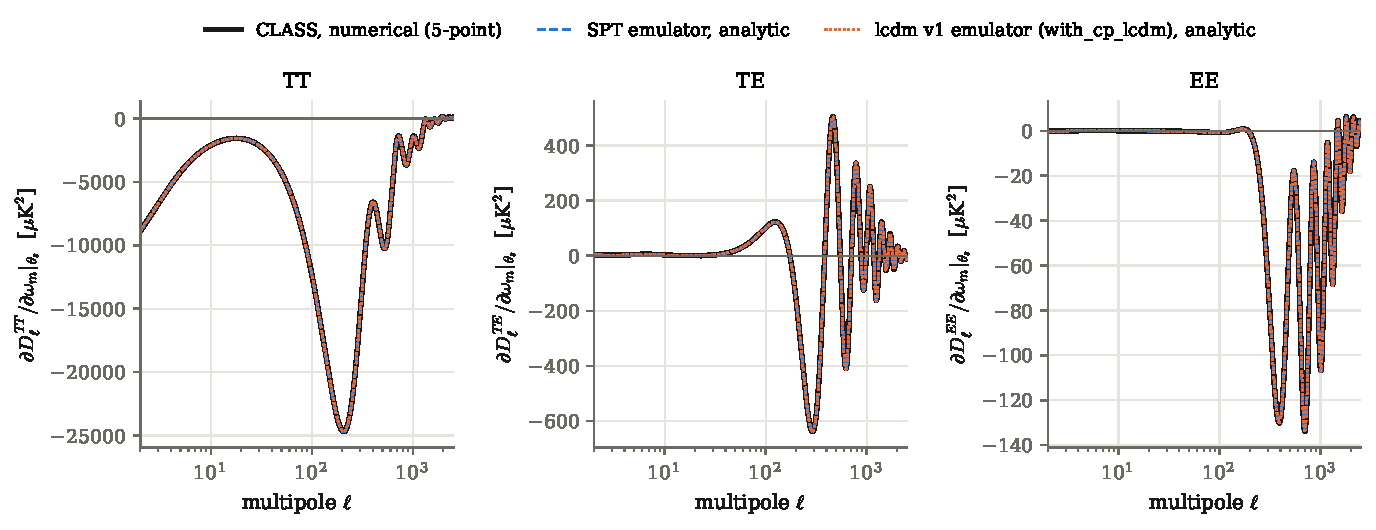
\includegraphics[width=\textwidth]{fig_derivs.pdf}
\caption{The derivative $\partial D_\ell/\partial\om|_{\theta_s}$, $D_\ell=\ell(\ell+1)C_\ell/2\pi$, for $TT$, $TE$,
$EE$: CLASS (numerical, black), SPT emulator (analytic, blue dashed) and lcdm v1 emulator of the with\_cp\_lcdm
pipeline (analytic, orange dotted). The three are indistinguishable at this scale; differences in
Fig.~\ref{fig:err}.}
\label{fig:derivs}
\end{figure}

\begin{figure}[H]
\centering
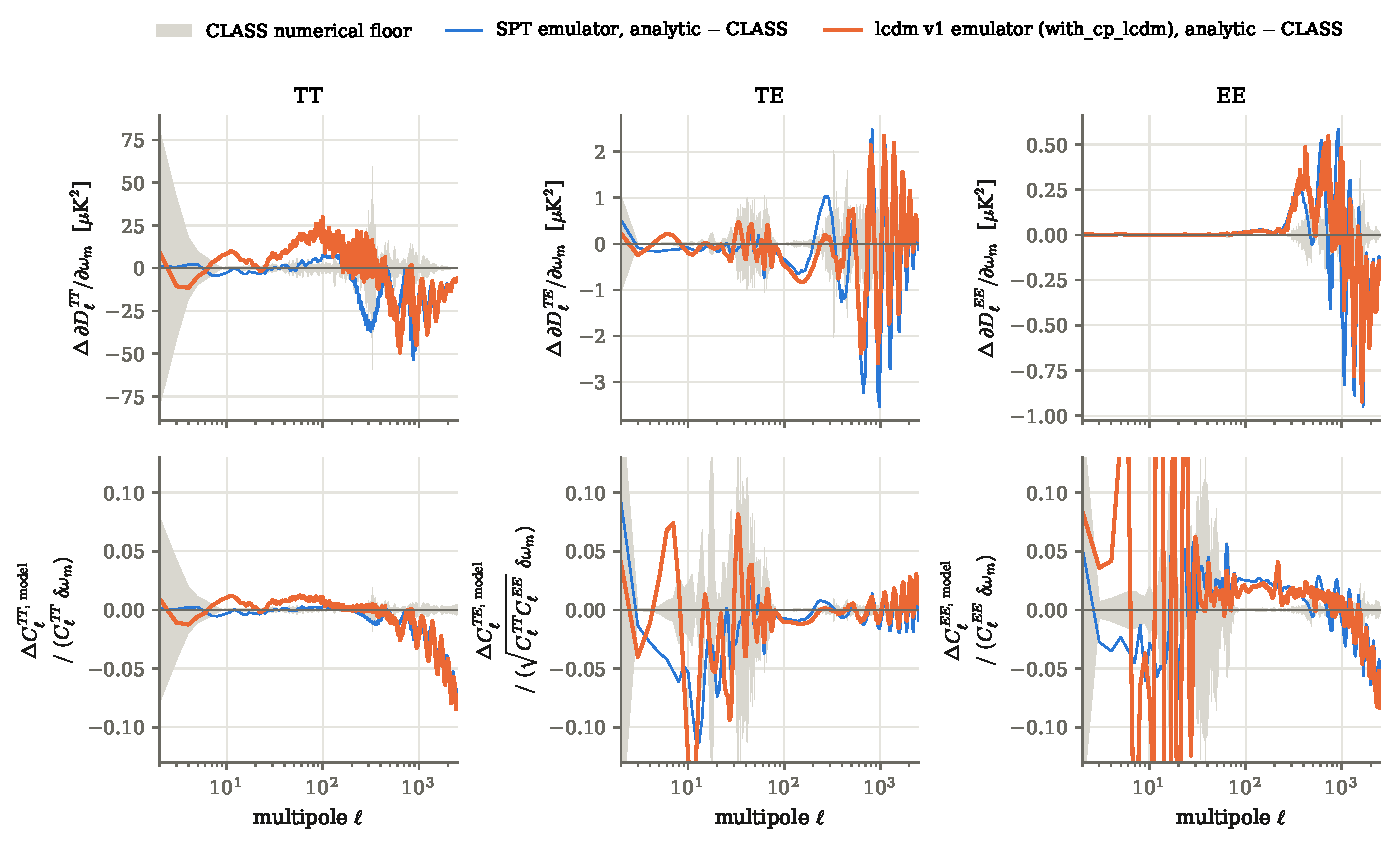
\includegraphics[width=\textwidth]{fig_errors.pdf}
\caption{Error of the \emph{analytic} emulator derivatives with respect to the CLASS benchmark.
\textbf{Top:} absolute, $\Delta\,\partial D_\ell/\partial\om$ in $\mu{\rm K}^2$ per unit $\om$.
\textbf{Bottom:} the resulting model error relative to the spectrum, $\Delta C_\ell^{\rm model}/(C_\ell\,\delta\om)
=\Delta(\dC)/C_\ell$ ($TE$: $/\sqrt{C^{TT}_\ell C^{EE}_\ell}$); multiply by $\delta\om$ to get $\Delta C_\ell^{\rm model}/C_\ell$.
Orange (thick): lcdm v1 emulator, analytic, exactly as computed inside the with\_cp\_lcdm pipeline
(\texttt{dcl\_domega\_m()}, fitted slope). Blue: SPT emulator, analytic. Grey band: CLASS numerical floor.
Off scale in the bottom row: lcdm v1 $TE$ at 2 multipoles with $\ell\le12$ (max $0.16$) and $EE$ at 13 multipoles
with $\ell\le24$ (max $0.71$), where $C_\ell^{EE}$ is at its minimum.}
\label{fig:err}
\end{figure}

\begin{figure}[H]
\centering
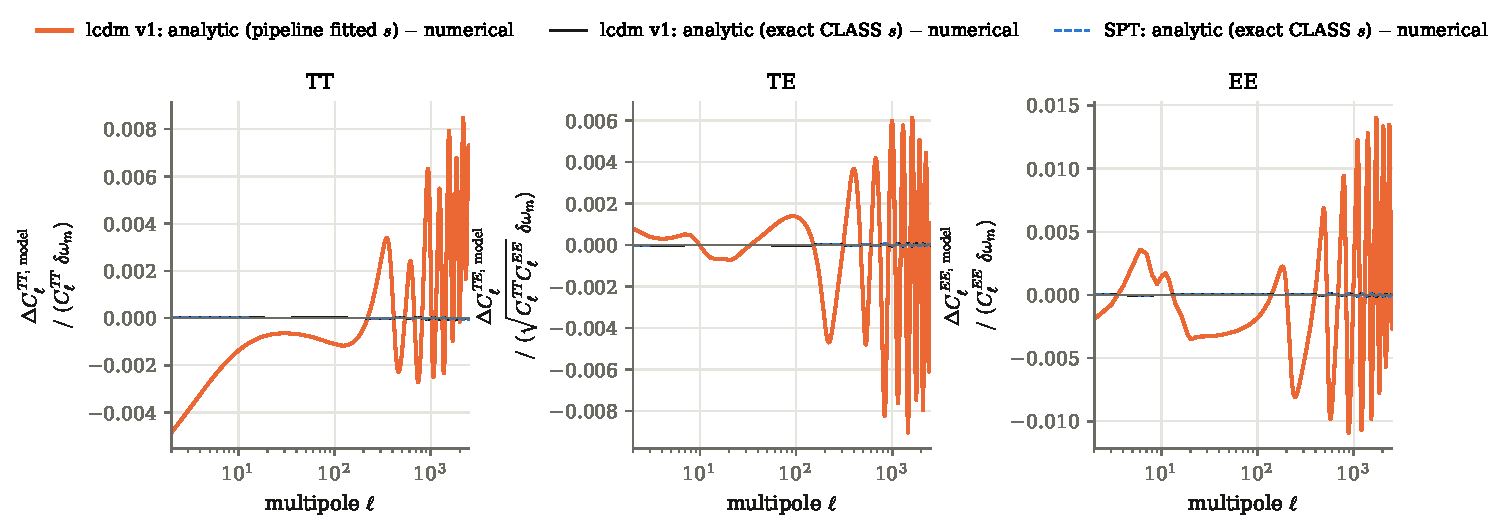
\includegraphics[width=\textwidth]{fig_an_vs_num.pdf}
\caption{Analytic minus numerical derivative of the \emph{same} emulator, as model error relative to the spectrum,
$\Delta C_\ell^{\rm model}/(C_\ell\,\delta\om)$.
With the exact CLASS slope $s=\sexact$ the analytic and numerical derivatives agree to $\lesssim10^{-4}$ for both
emulators (black and blue lines, on top of zero): the analytic Jacobians are exact. The orange line is the
pipeline's analytic derivative, which uses the fitted slope $s=\spipe$ ($0.1\%$ off): this alone shifts the
model by up to $0.008\,\delta\om$ ($TT$), $0.009\,\delta\om$ ($TE$) and $0.014\,\delta\om$ ($EE$) in units of $C_\ell$.}
\label{fig:anvsnum}
\end{figure}

\begin{table}[H]
\centering
\caption{Noise-weighted size of each model error for $\delta\om=\sigma(\om)=0.0012$ (scales linearly with $\delta\om$):
$\sqrt{\chi^2}=\big[\sum_\ell(\Delta\,\dC\,\delta\om)^2/{\rm Var}(C_\ell)\big]^{1/2}$, cosmic variance only,
$f_{\rm sky}=0.57$, $30\le\ell\le2508$. The first row is the size of the template itself.}
\label{tab:chi2}
\begin{tabular}{l S[table-format=1.3] S[table-format=1.3] S[table-format=1.3]}
\toprule
 & {TT} & {TE} & {EE} \\
\midrule
template itself (CLASS) & 2.041 & 1.921 & 3.043 \\
SPT analytic $-$ CLASS & 0.071 & 0.026 & 0.063 \\
lcdm v1 analytic (pipeline) $-$ CLASS & 0.080 & 0.030 & 0.067 \\
lcdm v1 analytic, exact $s$ $-$ CLASS & 0.086 & 0.036 & 0.073 \\
lcdm v1 analytic (pipeline) $-$ numerical & 0.007 & 0.010 & 0.012 \\
CLASS numerical floor & 0.005 & 0.006 & 0.009 \\
\bottomrule
\end{tabular}

\end{table}

\begin{table}[H]
\centering
\caption{$TT$: model error $\Delta C_\ell^{\rm model}/(C_\ell^{TT}\,\delta\om)$ in units of $10^{-2}$ (multiply by $\delta\om$ for the fractional change of $C_\ell^{TT}$). ``lcdm v1'' is the pipeline's analytic
derivative (fitted $s$), ``exact $s$'' the same with the exact CLASS slope.}
\label{tab:relTT}
\begin{tabular}{r S[table-format=-2.2] S[table-format=-2.2] S[table-format=-2.2] S[table-format=-2.3] S[table-format=-2.3] S[table-format=1.2]}
\toprule
& \multicolumn{3}{c}{analytic $-$ CLASS} & \multicolumn{2}{c}{analytic $-$ numerical} & {CLASS} \\
\cmidrule(lr){2-4}\cmidrule(lr){5-6}
{$\ell$} & {SPT} & {lcdm v1} & {lcdm v1, exact $s$} & {SPT} & {lcdm v1} & {floor} \\
\midrule
2 & 0.11 & 0.95 & 1.44 & 0.004 & -0.485 & 7.94 \\
10 & -0.32 & 1.02 & 1.16 & 0.001 & -0.137 & 0.09 \\
30 & -0.07 & 0.84 & 0.90 & 0.001 & -0.064 & 0.25 \\
100 & 0.28 & 1.11 & 1.22 & 0.001 & -0.111 & 0.12 \\
200 & -0.03 & 0.09 & 0.13 & 0.000 & -0.042 & 0.04 \\
500 & -0.39 & -0.71 & -0.56 & 0.001 & -0.152 & 0.22 \\
800 & -0.90 & -0.43 & -0.35 & 0.001 & -0.079 & 0.09 \\
1000 & -1.39 & -2.00 & -2.21 & -0.002 & 0.207 & 0.09 \\
1500 & -4.02 & -3.68 & -4.28 & -0.005 & 0.598 & 0.19 \\
2000 & -4.10 & -4.27 & -4.26 & 0.000 & -0.013 & 0.15 \\
2500 & -6.90 & -7.87 & -8.59 & -0.006 & 0.710 & 0.42 \\
\bottomrule
\end{tabular}

\end{table}

\begin{table}[H]
\centering
\caption{$TE$: model error $\Delta C_\ell^{\rm model}/(\sqrt{C_\ell^{TT}C_\ell^{EE}}\,\delta\om)$ in units of $10^{-2}$. Columns as in Table~\ref{tab:relTT}.}
\label{tab:relTE}
\begin{tabular}{r S[table-format=-2.2] S[table-format=-2.2] S[table-format=-2.2] S[table-format=-2.3] S[table-format=-2.3] S[table-format=1.2]}
\toprule
& \multicolumn{3}{c}{analytic $-$ CLASS} & \multicolumn{2}{c}{analytic $-$ numerical} & {CLASS} \\
\cmidrule(lr){2-4}\cmidrule(lr){5-6}
{$\ell$} & {SPT} & {lcdm v1} & {lcdm v1, exact $s$} & {SPT} & {lcdm v1} & {floor} \\
\midrule
2 & 9.25 & 4.01 & 3.93 & -0.001 & 0.081 & 18.70 \\
10 & -5.32 & -12.57 & -12.56 & 0.000 & -0.003 & 2.25 \\
30 & -3.05 & 0.24 & 0.26 & 0.000 & -0.016 & 2.66 \\
100 & -0.73 & -1.03 & -1.16 & -0.001 & 0.137 & 0.02 \\
200 & 0.01 & -0.79 & -0.40 & 0.003 & -0.385 & 0.12 \\
500 & 0.26 & 0.45 & 0.76 & 0.003 & -0.307 & 0.01 \\
800 & 1.00 & 0.86 & 1.46 & 0.005 & -0.596 & 0.17 \\
1000 & -1.27 & -0.47 & -1.07 & -0.005 & 0.596 & 0.11 \\
1500 & -0.03 & -0.24 & 0.34 & 0.005 & -0.572 & 0.19 \\
2000 & 1.39 & 2.27 & 2.32 & 0.000 & -0.044 & 0.03 \\
2500 & -0.81 & 0.62 & 0.58 & -0.000 & 0.046 & 0.06 \\
\bottomrule
\end{tabular}

\end{table}

\begin{table}[H]
\centering
\caption{$EE$: model error $\Delta C_\ell^{\rm model}/(C_\ell^{EE}\,\delta\om)$ in units of $10^{-2}$. Columns as in Table~\ref{tab:relTT}.}
\label{tab:relEE}
\begin{tabular}{r S[table-format=-2.2] S[table-format=-2.2] S[table-format=-2.2] S[table-format=-2.3] S[table-format=-2.3] S[table-format=1.2]}
\toprule
& \multicolumn{3}{c}{analytic $-$ CLASS} & \multicolumn{2}{c}{analytic $-$ numerical} & {CLASS} \\
\cmidrule(lr){2-4}\cmidrule(lr){5-6}
{$\ell$} & {SPT} & {lcdm v1} & {lcdm v1, exact $s$} & {SPT} & {lcdm v1} & {floor} \\
\midrule
2 & 5.27 & 8.39 & 8.58 & 0.002 & -0.192 & 16.60 \\
10 & -2.81 & -7.59 & -7.74 & -0.001 & 0.144 & 2.03 \\
30 & 2.41 & 6.18 & 6.52 & 0.003 & -0.329 & 4.68 \\
100 & 2.51 & 1.82 & 2.00 & 0.002 & -0.181 & 0.09 \\
200 & 1.97 & 1.72 & 1.69 & -0.000 & 0.035 & 0.18 \\
500 & -0.55 & 1.44 & 0.81 & -0.006 & 0.630 & 0.28 \\
800 & -1.44 & -0.40 & -1.29 & -0.008 & 0.887 & 0.43 \\
1000 & -1.12 & 0.03 & -0.09 & -0.001 & 0.114 & 0.64 \\
1500 & 1.17 & -0.73 & 0.11 & 0.007 & -0.828 & 0.81 \\
2000 & -6.37 & -5.67 & -6.82 & -0.010 & 1.140 & 0.26 \\
2500 & -5.26 & -7.82 & -7.56 & 0.002 & -0.257 & 0.33 \\
\bottomrule
\end{tabular}

\end{table}

\section{Summary}
\begin{itemize}
\item The CLASS benchmark is a fixed-$\theta_s$ derivative to $4\times10^{-9}$ in $100\,\theta_s$, with a numerical
  floor of $\sqrt{\chi^2}\le0.009$ (Table~\ref{tab:chi2}).
\item Both emulators reproduce it to $\sqrt{\chi^2}\approx0.03$--$0.09$ per $1\sigma$ shift, against a template of
  $\approx2$--$3$, i.e.\ to 1.5--4\%. The model error grows with $\ell$: $\Delta C_\ell^{TT,\rm model}/C_\ell^{TT}\approx-0.04\,\delta\om$ at
  $\ell=1500$--$2000$ and $-(0.07$--$0.08)\,\delta\om$ at $\ell=2500$, i.e.\ below $10^{-3}$ of $C_\ell$ at $\ell\ge30$ for any
  $|\delta\om|\lesssim0.01$, for both emulators (similar shape, so likely shared
  training/settings differences with respect to this CLASS run).
\item For the lcdm v1 (pipeline) derivative, the fitted slope $s$ accounts for a visible part of the difference
  (Fig.~\ref{fig:anvsnum}); here it happens to partly cancel the emulator error
  ($\sqrt{\chi^2}$ 0.080/0.030/0.067 with the fitted slope vs 0.086/0.036/0.073 with the exact one).
\end{itemize}

\appendix
\section{Values of the derivatives}

\begin{table}[H]
\centering\small
\caption{$TT$: $D_\ell$ and $\partial D_\ell/\partial\om|_{\theta_s}$ from the five methods ($\mu{\rm K}^2$).}
\begin{tabular}{r S[table-format=-1.3e1] S[table-format=-1.3e1] S[table-format=-1.3e1] S[table-format=-1.3e1] S[table-format=-1.3e1] S[table-format=-1.3e1]}
\toprule
{$\ell$} & {$D_\ell^{TT}$} & {CLASS} & {SPT num.} & {SPT anal.} & {lcdm v1 num.} & {lcdm v1 anal.} \\
 & {[$\mu$K$^2$]} & \multicolumn{5}{c}{$\partial D_\ell^{TT}/\partial\omega_m|_{\theta_s}$ [$\mu$K$^2$]} \\
\midrule
2 & 1.022e+03 & -8.890e+03 & -8.889e+03 & -8.889e+03 & -8.875e+03 & -8.880e+03 \\
10 & 8.195e+02 & -2.112e+03 & -2.115e+03 & -2.115e+03 & -2.103e+03 & -2.104e+03 \\
30 & 1.057e+03 & -2.132e+03 & -2.133e+03 & -2.133e+03 & -2.123e+03 & -2.123e+03 \\
100 & 2.703e+03 & -1.234e+04 & -1.233e+04 & -1.233e+04 & -1.231e+04 & -1.231e+04 \\
200 & 5.607e+03 & -2.464e+04 & -2.464e+04 & -2.464e+04 & -2.464e+04 & -2.464e+04 \\
500 & 2.448e+03 & -9.947e+03 & -9.957e+03 & -9.957e+03 & -9.961e+03 & -9.964e+03 \\
800 & 2.526e+03 & -2.893e+03 & -2.916e+03 & -2.916e+03 & -2.902e+03 & -2.904e+03 \\
1000 & 1.062e+03 & -1.437e+03 & -1.451e+03 & -1.451e+03 & -1.460e+03 & -1.458e+03 \\
1500 & 6.880e+02 & -6.203e+02 & -6.479e+02 & -6.479e+02 & -6.497e+02 & -6.456e+02 \\
2000 & 2.312e+02 & 8.479e+01 & 7.530e+01 & 7.530e+01 & 7.494e+01 & 7.491e+01 \\
2500 & 7.864e+01 & 8.144e+01 & 7.602e+01 & 7.601e+01 & 7.469e+01 & 7.525e+01 \\
\bottomrule
\end{tabular}

\end{table}
\begin{table}[H]
\centering\small
\caption{$TE$: $D_\ell$ and $\partial D_\ell/\partial\om|_{\theta_s}$ from the five methods ($\mu{\rm K}^2$).}
\begin{tabular}{r S[table-format=-1.3e1] S[table-format=-1.3e1] S[table-format=-1.3e1] S[table-format=-1.3e1] S[table-format=-1.3e1] S[table-format=-1.3e1]}
\toprule
{$\ell$} & {$D_\ell^{TE}$} & {CLASS} & {SPT num.} & {SPT anal.} & {lcdm v1 num.} & {lcdm v1 anal.} \\
 & {[$\mu$K$^2$]} & \multicolumn{5}{c}{$\partial D_\ell^{TE}/\partial\omega_m|_{\theta_s}$ [$\mu$K$^2$]} \\
\midrule
2 & 2.619e+00 & 2.951e+00 & 3.469e+00 & 3.469e+00 & 3.171e+00 & 3.175e+00 \\
10 & 8.435e-01 & 2.652e+00 & 2.568e+00 & 2.568e+00 & 2.453e+00 & 2.453e+00 \\
30 & 1.891e+00 & 3.012e+00 & 2.866e+00 & 2.866e+00 & 3.024e+00 & 3.023e+00 \\
100 & -2.317e+01 & 1.025e+02 & 1.021e+02 & 1.021e+02 & 1.019e+02 & 1.020e+02 \\
200 & -1.537e+01 & -1.611e+02 & -1.611e+02 & -1.611e+02 & -1.613e+02 & -1.616e+02 \\
500 & -5.863e+01 & 3.718e+02 & 3.722e+02 & 3.722e+02 & 3.729e+02 & 3.725e+02 \\
800 & -8.893e+01 & 3.166e+02 & 3.186e+02 & 3.186e+02 & 3.195e+02 & 3.183e+02 \\
1000 & -2.427e+01 & 5.149e+01 & 4.882e+01 & 4.881e+01 & 4.923e+01 & 5.049e+01 \\
1500 & -4.459e-01 & -7.132e+00 & -7.161e+00 & -7.156e+00 & -6.820e+00 & -7.356e+00 \\
2000 & -1.804e+01 & 3.044e+01 & 3.106e+01 & 3.107e+01 & 3.148e+01 & 3.146e+01 \\
2500 & -2.935e+00 & -1.396e+01 & -1.408e+01 & -1.408e+01 & -1.387e+01 & -1.387e+01 \\
\bottomrule
\end{tabular}

\end{table}
\begin{table}[H]
\centering\small
\caption{$EE$: $D_\ell$ and $\partial D_\ell/\partial\om|_{\theta_s}$ from the five methods ($\mu{\rm K}^2$).}
\begin{tabular}{r S[table-format=-1.3e1] S[table-format=-1.3e1] S[table-format=-1.3e1] S[table-format=-1.3e1] S[table-format=-1.3e1] S[table-format=-1.3e1]}
\toprule
{$\ell$} & {$D_\ell^{EE}$} & {CLASS} & {SPT num.} & {SPT anal.} & {lcdm v1 num.} & {lcdm v1 anal.} \\
 & {[$\mu$K$^2$]} & \multicolumn{5}{c}{$\partial D_\ell^{EE}/\partial\omega_m|_{\theta_s}$ [$\mu$K$^2$]} \\
\midrule
2 & 3.079e-02 & -2.057e-01 & -2.041e-01 & -2.041e-01 & -2.031e-01 & -2.031e-01 \\
10 & 3.052e-03 & 2.132e-02 & 2.123e-02 & 2.123e-02 & 2.108e-02 & 2.109e-02 \\
30 & 2.155e-02 & -4.375e-02 & -4.323e-02 & -4.323e-02 & -4.234e-02 & -4.241e-02 \\
100 & 7.769e-01 & -8.172e-01 & -7.977e-01 & -7.977e-01 & -8.016e-01 & -8.030e-01 \\
200 & 6.896e-01 & -1.002e+00 & -9.883e-01 & -9.883e-01 & -9.902e-01 & -9.900e-01 \\
500 & 8.315e+00 & -3.937e+01 & -3.942e+01 & -3.942e+01 & -3.930e+01 & -3.925e+01 \\
800 & 1.559e+01 & -4.662e+01 & -4.684e+01 & -4.684e+01 & -4.682e+01 & -4.668e+01 \\
1000 & 4.213e+01 & -1.064e+02 & -1.069e+02 & -1.069e+02 & -1.065e+02 & -1.064e+02 \\
1500 & 1.272e+01 & 3.386e+00 & 3.534e+00 & 3.535e+00 & 3.399e+00 & 3.293e+00 \\
2000 & 8.634e+00 & -1.190e+01 & -1.245e+01 & -1.245e+01 & -1.249e+01 & -1.239e+01 \\
2500 & 2.896e+00 & 1.370e+00 & 1.217e+00 & 1.217e+00 & 1.151e+00 & 1.143e+00 \\
\bottomrule
\end{tabular}

\end{table}

\section{Files}
\texttt{debug/dcl\_domegam\_spt\_vs\_class/}: \texttt{compute\_derivs.py} (CLASS + SPT, $\sim$35 min on 2 cores),
\texttt{compute\_v1.py} (lcdm v1 through the pipeline's \texttt{classy.py}), \texttt{theta\_check.py},
\texttt{make\_report.py} (figures and tables), \texttt{spt\_emu.py} (numpy SPT networks with exact Jacobian),
\texttt{cpstub/} (numpy stand-in for \texttt{cosmopower}, only needed without TensorFlow), \texttt{*.npz} (all
derivatives).
\end{document}
